\documentclass{article}

\usepackage{Sweave}
\begin{document}
\Sconcordance{concordance:BtheBteam1.tex:BtheBteam1.Rnw:%
1 2 1 1 0 17 1 1 2 1 0 2 1 1 2 2 1 21 0 1 2 1 8 1 2 8 1 1 40 1 2 1 0 2 %
1 4 0 1 2 2 1 1 2 1 0 2 1 22 0 3 1 23 0 1 1 25 0 1 2 4 1 1 10 6 0 1 2 2 %
0 1 2 2 0 1 1 3 0 1 2 16 1}

\title{Write-up for the Beat the Blues Data}
\author{Eric Reed, Sara Nunez, Yiding Zhang, Kostis Gourgoulias\\
University of Massachusetts, Amherst}
\maketitle
\newpage
\section{Background}
This is a dataset containing information from a clinical trial with "Beat the Blues", an interactive
multimedia program of cognitive-behavioural techniques. Since there are way more patients suffering from anxiety
and depression than therapists, the study of the dataset makes the case that this program can indeed help with
the treatment. One of the metrics used to gauge depression levels was BDI or Beck Depression Inventory.

The dataset contains one hundred observations of one hundred patients and eight variables.
BDI was tracked before treatment, after two months and then after one, three and six month follow-ups.
Two groups are studied, one that uses the BtB program and one that has the usual anti-depression treatment.
Those can be further splitted to sub-groups of patients that were taking anti-depressant drugs.

\begin{Schunk}
\begin{Sinput}
> library(ggplot2)
> library(MASS)
> library(HSAUR2)
> BtheB <- BtheB
> attach(BtheB)
> summary(BtheB)
\end{Sinput}
\begin{Soutput}
  drug    length   treatment     bdi.pre          bdi.2m          bdi.3m     
 No :56   <6m:49   TAU  :48   Min.   : 2.00   Min.   : 0.00   Min.   : 0.00  
 Yes:44   >6m:51   BtheB:52   1st Qu.:15.00   1st Qu.: 8.00   1st Qu.: 6.00  
                              Median :22.00   Median :15.00   Median :13.00  
                              Mean   :23.33   Mean   :16.92   Mean   :14.81  
                              3rd Qu.:30.25   3rd Qu.:23.00   3rd Qu.:20.00  
                              Max.   :49.00   Max.   :48.00   Max.   :53.00  
                                              NA's   :3       NA's   :27     
     bdi.5m          bdi.8m     
 Min.   : 0.00   Min.   : 0.00  
 1st Qu.: 3.00   1st Qu.: 3.00  
 Median :10.00   Median :10.50  
 Mean   :12.76   Mean   :11.13  
 3rd Qu.:20.00   3rd Qu.:15.25  
 Max.   :47.00   Max.   :40.00  
 NA's   :42      NA's   :48     
\end{Soutput}
\end{Schunk}

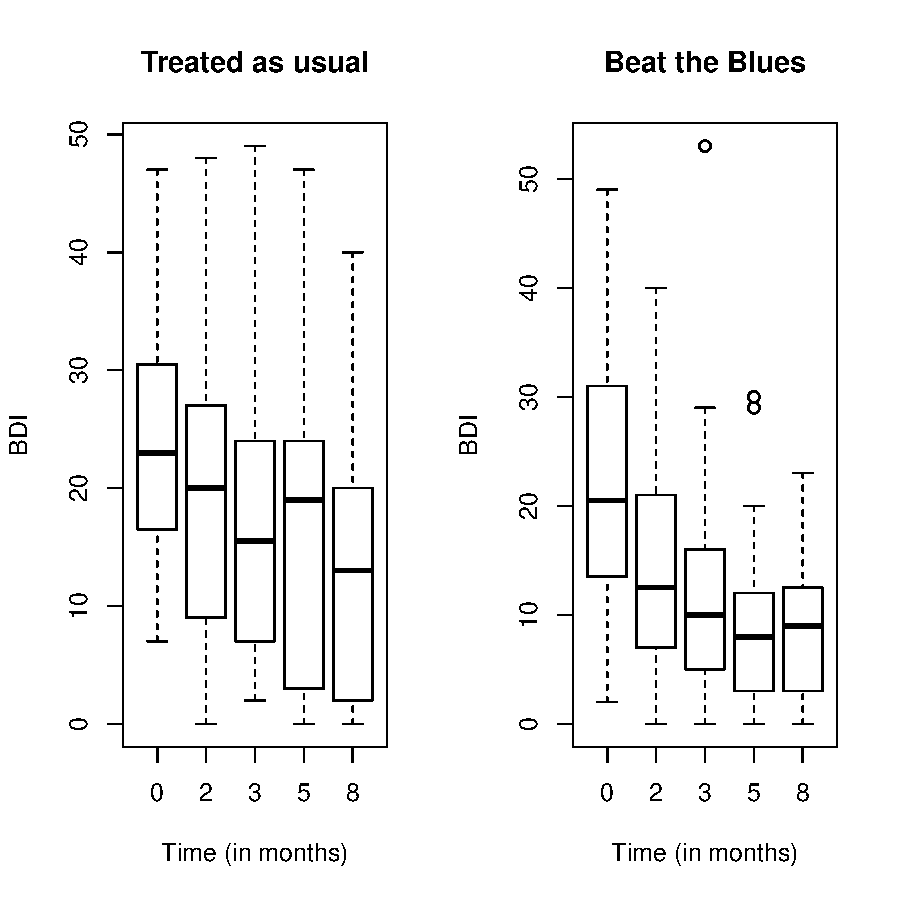
\includegraphics{BtheBteam1-002}
\section{Variables and Hypothesis}

The variables we chose to work with were bdi.2m and bdi.3m, which were the Beck Depression Inventory II test results of the 100 patients after two months and after three months, respectively.

The purpose of this analysis was to intperpret the results from a linear regression for the Beck Depression Inventory II test at week 3 as, a function of week 2. The slope of the regression line for this data, represents the proportion between the BDI at week 3 and week 2. We therefore hypothesize, that the slope of the regression line for the subset of the patients who recieved the "BtheB" treatment, will be smaller than that of the patients who recieved the "TAU" treatment. 
\newline
\newline
The following summarizes the two variables of interest for the usual treatment group and the beat the blues group:


\begin{Schunk}
\begin{Sinput}
> h1 = qplot(bdi.2m, fill = treatment, main ="BDI 2 month Follow-up Histogram")
> h2 = qplot(bdi.3m, fill = treatment, main ="BDI 3 month Follow-up Histogram")
> multiplot(h1,h2)
\end{Sinput}
\end{Schunk}
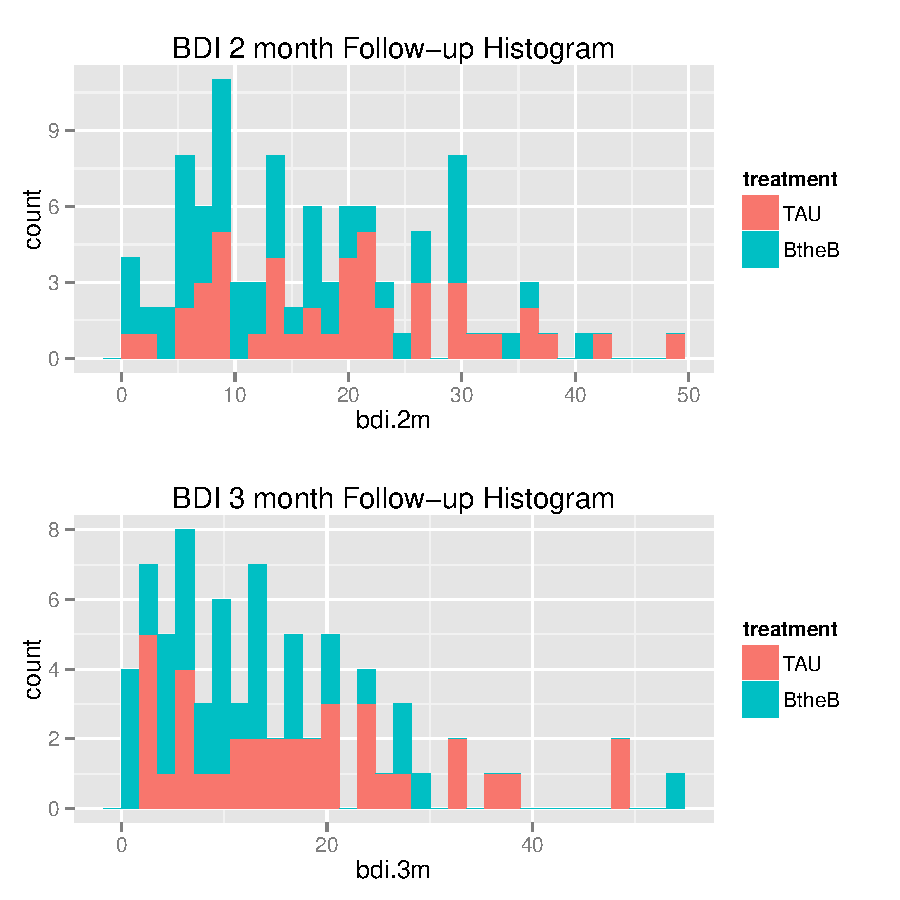
\includegraphics{BtheBteam1-004}



\begin{Schunk}
\begin{Sinput}
> qplot(bdi.2m,bdi.3m,data=BtheB, geom=c("point","smooth"),method="lm",color=treatment)
> m2m3m <- lm(bdi.3m~bdi.2m,data=BtheB)
> summary(m2m3m)
\end{Sinput}
\begin{Soutput}
Call:
lm(formula = bdi.3m ~ bdi.2m, data = BtheB)

Residuals:
     Min       1Q   Median       3Q      Max 
-24.2614  -4.6967  -0.3375   2.5850  22.5343 

Coefficients:
            Estimate Std. Error t value Pr(>|t|)    
(Intercept)  0.97839    1.53213   0.639    0.525    
bdi.2m       0.87183    0.08021  10.870   <2e-16 ***
---
Signif. codes:  0 ‘***’ 0.001 ‘**’ 0.01 ‘*’ 0.05 ‘.’ 0.1 ‘ ’ 1

Residual standard error: 7.293 on 71 degrees of freedom
  (27 observations deleted due to missingness)
Multiple R-squared:  0.6246,	Adjusted R-squared:  0.6193 
F-statistic: 118.1 on 1 and 71 DF,  p-value: < 2.2e-16
\end{Soutput}
\begin{Sinput}
> tau<-lm(bdi.3m&treatment=="TAU"~bdi.2m&treatment=="TAU", data=BtheB)
> btb<-lm(bdi.3m&treatment=="BtheB"~bdi.2m&treatment=="BtheB", data=BtheB)
> summary(tau)
\end{Sinput}
\begin{Soutput}
Call:
lm(formula = bdi.3m & treatment == "TAU" ~ bdi.2m & treatment == 
    "TAU", data = BtheB)

Residuals:
     Min       1Q   Median       3Q      Max 
-0.01887 -0.01887 -0.01887  0.00000  0.98113 

Coefficients:
                                Estimate Std. Error t value Pr(>|t|)    
(Intercept)                      0.01887    0.01467   1.286    0.202    
bdi.2m & treatment == "TAU"TRUE  0.98113    0.02326  42.174   <2e-16 ***
---
Signif. codes:  0 ‘***’ 0.001 ‘**’ 0.01 ‘*’ 0.05 ‘.’ 0.1 ‘ ’ 1

Residual standard error: 0.1068 on 86 degrees of freedom
  (12 observations deleted due to missingness)
Multiple R-squared:  0.9539,	Adjusted R-squared:  0.9533 
F-statistic:  1779 on 1 and 86 DF,  p-value: < 2.2e-16
\end{Soutput}
\begin{Sinput}
> summary(btb)
\end{Sinput}
\begin{Soutput}
Call:
lm(formula = bdi.3m & treatment == "BtheB" ~ bdi.2m & treatment == 
    "BtheB", data = BtheB)

Residuals:
     Min       1Q   Median       3Q      Max 
-0.94444  0.00000  0.00000  0.05556  0.05556 

Coefficients:
                                   Estimate Std. Error t value Pr(>|t|)    
(Intercept)                       7.707e-16  2.155e-02    0.00        1    
bdi.2m & treatment == "BtheB"TRUE 9.444e-01  3.311e-02   28.52   <2e-16 ***
---
Signif. codes:  0 ‘***’ 0.001 ‘**’ 0.01 ‘*’ 0.05 ‘.’ 0.1 ‘ ’ 1

Residual standard error: 0.1509 on 83 degrees of freedom
  (15 observations deleted due to missingness)
Multiple R-squared:  0.9074,	Adjusted R-squared:  0.9063 
F-statistic: 813.4 on 1 and 83 DF,  p-value: < 2.2e-16
\end{Soutput}
\end{Schunk}
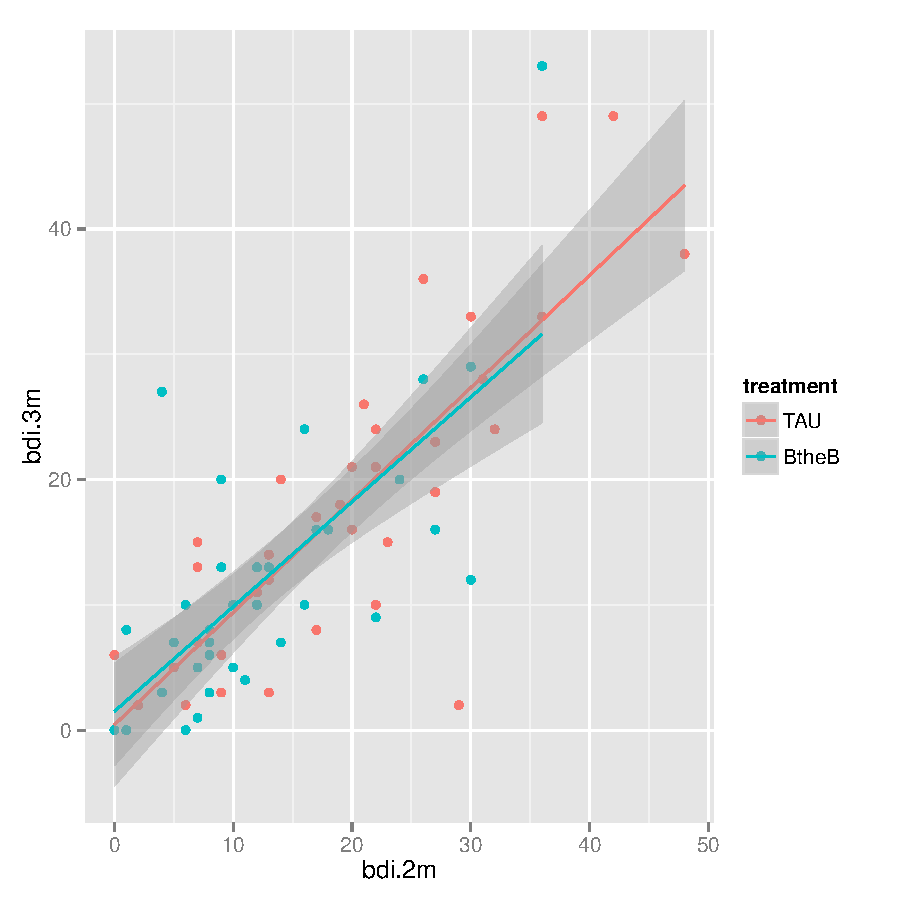
\includegraphics{BtheBteam1-005}



\section{Missing Data}

\begin{Schunk}
\begin{Soutput}
      bdi.2m bdi.3m Both
TAU        3     12    3
BtheB      0     15    0
Total      3     27    3
\end{Soutput}
\begin{Soutput}
[1] 73
\end{Soutput}
\begin{Soutput}
[1] 36
\end{Soutput}
\begin{Soutput}
[1] 37
\end{Soutput}
\end{Schunk}
There was missing data from 3 of the participants from week two and 27 from week three.  All 3 of the participants who had missing data from week two recieved the "TAU" treatment.  Of the 27 participants who had missing data from week three, 12 recieved the "TAU" treatment and 15 recieved the "BtheB" treatment.  All 3 of the missing participants from week two were also missing from week three, therefore a total of 27 patients are not included in our analysis, 12 from "TAU" and 15 from "BtheB", giving us 36 and 37 respective participants from each group.  A sample size of only 73, is certainly very small, and will be detrimental to the confidence we have in the outcome.  However, we have considerably more data on studay participants than if we had used data from week 5, or week 8, as each had missing data for 42 and 48 participants respectively.

\section{Results and Interpretation}

The regression line for the whole dataset had a $\beta$ value of 0.8718, and a correlational coefficient of 0.625.  The regression line for the subset of the data for paricipants in the "TAU" treatment group had a $\beta$  value of 0.9811, and had a correlational coeficcient of 0.954. The regression line for the subset of the data for paricipants in the "BtheB" treatment group had a $\beta$  value of 0.944, and had a correlational coeficcient of 0.907.
We can interpret these results to say that for the whole datset, given a one unit increase in bdi.2w we can expect a 0.8718 unit increase in bdi.3w.  For the subset containing partipants who underwent the "TAU" treatment, given a 1 unit increase in bdi.2w we can expect a 0.9811 unit increase in bdi.3w. And, For the subset containing partipants who underwent the "BtheB" treatment, given a 1 unit increase in bdi.2w we can expect a 0.944 unit increase in bdi.3w.  This supports our hypothesis since the proportion, $\beta$ value, between our before, "bdi,2w", and after, "bdi.3w", is smaller for the "BtheB" group.

It should also be noted that our regression lines proved to be a much better predictor when we subsetted the data, as the correlational coefficients are much close to 1 for the each subset than the whole dataset.


\begin{thebibliography}{1}
\bibitem{Proudfoot}
J. Proudfoot, D. Goldberg, A. Mann, B. S. Everitt, I. Marks and J. A. Gray, (2003). Computerized, interactive, multimedia cognitive-behavioural program for anxiety and depression in general practice. Psychological Medicine, 33(2), 217–227.*
\end{thebibliography}


\end{document}
